% Options for packages loaded elsewhere
\PassOptionsToPackage{unicode}{hyperref}
\PassOptionsToPackage{hyphens}{url}
%
\documentclass[
]{article}
\usepackage{amsmath,amssymb}
\usepackage{lmodern}
\usepackage{iftex}
\ifPDFTeX
  \usepackage[T1]{fontenc}
  \usepackage[utf8]{inputenc}
  \usepackage{textcomp} % provide euro and other symbols
\else % if luatex or xetex
  \usepackage{unicode-math}
  \defaultfontfeatures{Scale=MatchLowercase}
  \defaultfontfeatures[\rmfamily]{Ligatures=TeX,Scale=1}
\fi
% Use upquote if available, for straight quotes in verbatim environments
\IfFileExists{upquote.sty}{\usepackage{upquote}}{}
\IfFileExists{microtype.sty}{% use microtype if available
  \usepackage[]{microtype}
  \UseMicrotypeSet[protrusion]{basicmath} % disable protrusion for tt fonts
}{}
\makeatletter
\@ifundefined{KOMAClassName}{% if non-KOMA class
  \IfFileExists{parskip.sty}{%
    \usepackage{parskip}
  }{% else
    \setlength{\parindent}{0pt}
    \setlength{\parskip}{6pt plus 2pt minus 1pt}}
}{% if KOMA class
  \KOMAoptions{parskip=half}}
\makeatother
\usepackage{xcolor}
\usepackage[margin=1in]{geometry}
\usepackage{color}
\usepackage{fancyvrb}
\newcommand{\VerbBar}{|}
\newcommand{\VERB}{\Verb[commandchars=\\\{\}]}
\DefineVerbatimEnvironment{Highlighting}{Verbatim}{commandchars=\\\{\}}
% Add ',fontsize=\small' for more characters per line
\usepackage{framed}
\definecolor{shadecolor}{RGB}{248,248,248}
\newenvironment{Shaded}{\begin{snugshade}}{\end{snugshade}}
\newcommand{\AlertTok}[1]{\textcolor[rgb]{0.94,0.16,0.16}{#1}}
\newcommand{\AnnotationTok}[1]{\textcolor[rgb]{0.56,0.35,0.01}{\textbf{\textit{#1}}}}
\newcommand{\AttributeTok}[1]{\textcolor[rgb]{0.77,0.63,0.00}{#1}}
\newcommand{\BaseNTok}[1]{\textcolor[rgb]{0.00,0.00,0.81}{#1}}
\newcommand{\BuiltInTok}[1]{#1}
\newcommand{\CharTok}[1]{\textcolor[rgb]{0.31,0.60,0.02}{#1}}
\newcommand{\CommentTok}[1]{\textcolor[rgb]{0.56,0.35,0.01}{\textit{#1}}}
\newcommand{\CommentVarTok}[1]{\textcolor[rgb]{0.56,0.35,0.01}{\textbf{\textit{#1}}}}
\newcommand{\ConstantTok}[1]{\textcolor[rgb]{0.00,0.00,0.00}{#1}}
\newcommand{\ControlFlowTok}[1]{\textcolor[rgb]{0.13,0.29,0.53}{\textbf{#1}}}
\newcommand{\DataTypeTok}[1]{\textcolor[rgb]{0.13,0.29,0.53}{#1}}
\newcommand{\DecValTok}[1]{\textcolor[rgb]{0.00,0.00,0.81}{#1}}
\newcommand{\DocumentationTok}[1]{\textcolor[rgb]{0.56,0.35,0.01}{\textbf{\textit{#1}}}}
\newcommand{\ErrorTok}[1]{\textcolor[rgb]{0.64,0.00,0.00}{\textbf{#1}}}
\newcommand{\ExtensionTok}[1]{#1}
\newcommand{\FloatTok}[1]{\textcolor[rgb]{0.00,0.00,0.81}{#1}}
\newcommand{\FunctionTok}[1]{\textcolor[rgb]{0.00,0.00,0.00}{#1}}
\newcommand{\ImportTok}[1]{#1}
\newcommand{\InformationTok}[1]{\textcolor[rgb]{0.56,0.35,0.01}{\textbf{\textit{#1}}}}
\newcommand{\KeywordTok}[1]{\textcolor[rgb]{0.13,0.29,0.53}{\textbf{#1}}}
\newcommand{\NormalTok}[1]{#1}
\newcommand{\OperatorTok}[1]{\textcolor[rgb]{0.81,0.36,0.00}{\textbf{#1}}}
\newcommand{\OtherTok}[1]{\textcolor[rgb]{0.56,0.35,0.01}{#1}}
\newcommand{\PreprocessorTok}[1]{\textcolor[rgb]{0.56,0.35,0.01}{\textit{#1}}}
\newcommand{\RegionMarkerTok}[1]{#1}
\newcommand{\SpecialCharTok}[1]{\textcolor[rgb]{0.00,0.00,0.00}{#1}}
\newcommand{\SpecialStringTok}[1]{\textcolor[rgb]{0.31,0.60,0.02}{#1}}
\newcommand{\StringTok}[1]{\textcolor[rgb]{0.31,0.60,0.02}{#1}}
\newcommand{\VariableTok}[1]{\textcolor[rgb]{0.00,0.00,0.00}{#1}}
\newcommand{\VerbatimStringTok}[1]{\textcolor[rgb]{0.31,0.60,0.02}{#1}}
\newcommand{\WarningTok}[1]{\textcolor[rgb]{0.56,0.35,0.01}{\textbf{\textit{#1}}}}
\usepackage{graphicx}
\makeatletter
\def\maxwidth{\ifdim\Gin@nat@width>\linewidth\linewidth\else\Gin@nat@width\fi}
\def\maxheight{\ifdim\Gin@nat@height>\textheight\textheight\else\Gin@nat@height\fi}
\makeatother
% Scale images if necessary, so that they will not overflow the page
% margins by default, and it is still possible to overwrite the defaults
% using explicit options in \includegraphics[width, height, ...]{}
\setkeys{Gin}{width=\maxwidth,height=\maxheight,keepaspectratio}
% Set default figure placement to htbp
\makeatletter
\def\fps@figure{htbp}
\makeatother
\setlength{\emergencystretch}{3em} % prevent overfull lines
\providecommand{\tightlist}{%
  \setlength{\itemsep}{0pt}\setlength{\parskip}{0pt}}
\setcounter{secnumdepth}{-\maxdimen} % remove section numbering
\ifLuaTeX
  \usepackage{selnolig}  % disable illegal ligatures
\fi
\IfFileExists{bookmark.sty}{\usepackage{bookmark}}{\usepackage{hyperref}}
\IfFileExists{xurl.sty}{\usepackage{xurl}}{} % add URL line breaks if available
\urlstyle{same} % disable monospaced font for URLs
\hypersetup{
  pdftitle={Task: Facets},
  pdfauthor={Mansi Patel},
  hidelinks,
  pdfcreator={LaTeX via pandoc}}

\title{Task: Facets}
\author{Mansi Patel}
\date{2022-10-07}

\begin{document}
\maketitle

The goal of this task is to practice the use of facets in
visualizations. For each question you are asked to make a visualization
using facets. Be sure to use \texttt{facet\_wrap} for at least one plot
and \texttt{facet\_grid} for at least one plot.

Use the subset of the \texttt{diamonds} dataset defined below.

\begin{Shaded}
\begin{Highlighting}[]
\NormalTok{diamonds\_subset }\OtherTok{\textless{}{-}}\NormalTok{ diamonds }\SpecialCharTok{|\textgreater{}} \FunctionTok{filter}\NormalTok{(clarity }\SpecialCharTok{==} \StringTok{"IF"}\NormalTok{, carat }\SpecialCharTok{\textgreater{}} \FloatTok{0.5}\NormalTok{)}
\end{Highlighting}
\end{Shaded}

\hypertarget{question-1}{%
\subsection{Question 1}\label{question-1}}

Make a scatter plot of price as a function of carat from the
\texttt{diamonds\_subset} data. Create a facet for each level of the
\texttt{cut} categorical variable.

\begin{Shaded}
\begin{Highlighting}[]
\CommentTok{\#|The following visualisation represents variation of price and carat of diamonds of different cut type}
\NormalTok{diamonds\_subset }\SpecialCharTok{|\textgreater{}} \FunctionTok{ggplot}\NormalTok{(}\FunctionTok{aes}\NormalTok{(}\AttributeTok{y=}\NormalTok{price, }\AttributeTok{x=}\NormalTok{carat, }\AttributeTok{color =}\NormalTok{ cut)) }\SpecialCharTok{+} \FunctionTok{geom\_point}\NormalTok{() }\SpecialCharTok{+} \FunctionTok{facet\_wrap}\NormalTok{(}\SpecialCharTok{\textasciitilde{}}\NormalTok{cut);}
\end{Highlighting}
\end{Shaded}

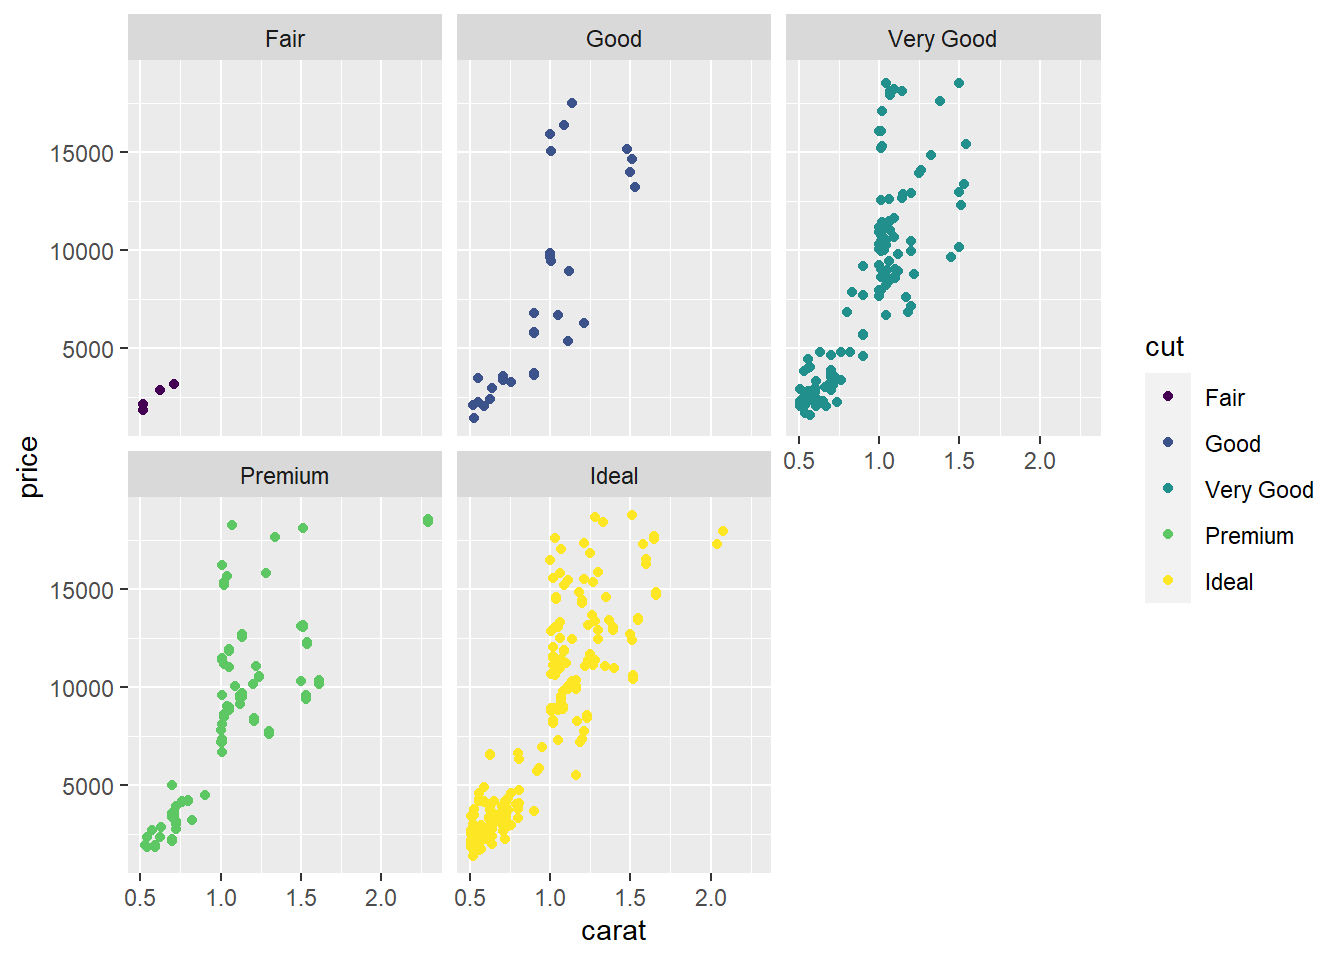
\includegraphics{task-facets_files/figure-latex/unnamed-chunk-2-1.pdf}

We can see from the graph that scatter plot that the diamonds with ideal
cut or very good cut has very similar relation between price and carat.
In all types of cut if the diamond is near 0.5 carat it will have price
less than 5000. \#\# Question 2

Make a scatter plot of the length and width of each diamond (the
variables \texttt{x} and \texttt{y}) in the diamonds subset data. Create
facets for each combination of \texttt{color} and \texttt{cut}.

\begin{Shaded}
\begin{Highlighting}[]
\NormalTok{diamonds\_subset }\SpecialCharTok{|\textgreater{}} \FunctionTok{ggplot}\NormalTok{(}\FunctionTok{aes}\NormalTok{ (x, y, }\AttributeTok{color =}\NormalTok{ cut)) }\SpecialCharTok{+} \FunctionTok{geom\_point}\NormalTok{() }\SpecialCharTok{+} \FunctionTok{facet\_grid}\NormalTok{(cut }\SpecialCharTok{\textasciitilde{}}\NormalTok{ color, }\AttributeTok{labeller =} \FunctionTok{labeller}\NormalTok{(}\AttributeTok{.cols =} \ControlFlowTok{function}\NormalTok{(x) }\FunctionTok{paste}\NormalTok{(x,}\StringTok{"color"}\NormalTok{), }\AttributeTok{.rows =} \ControlFlowTok{function}\NormalTok{(y) }\FunctionTok{paste}\NormalTok{(y,}\StringTok{"cut"}\NormalTok{)))}
\end{Highlighting}
\end{Shaded}

\begin{figure}
\centering
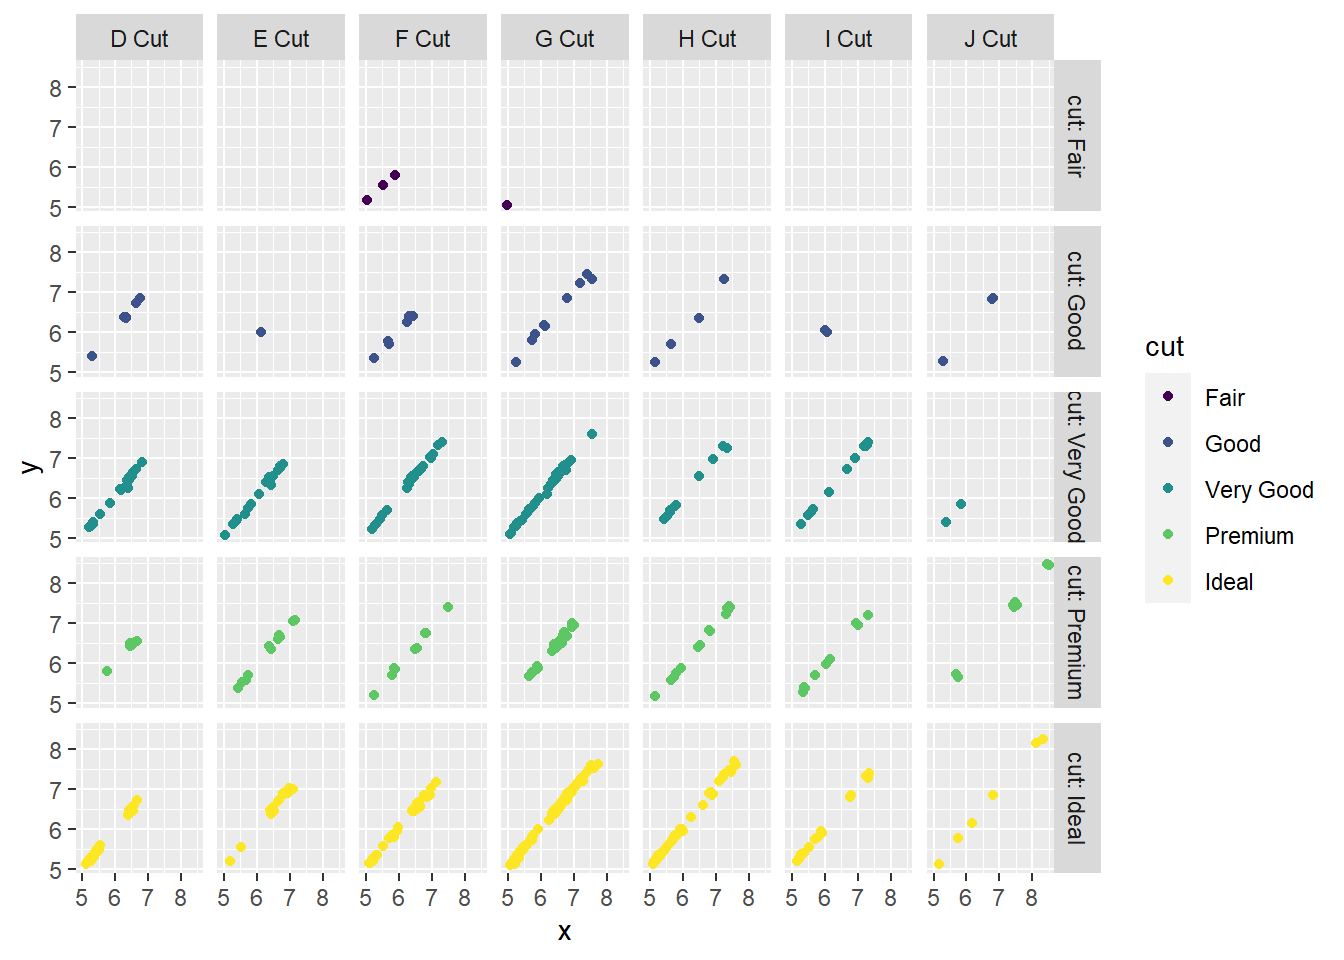
\includegraphics{task-facets_files/figure-latex/unnamed-chunk-3-1.pdf}
\caption{the visualization represents relation between length and width
of diamonds of different color and cuts}
\end{figure}

This graph represents linear relation between x and y variables. It also
shows that for very good, premium and Ideal cut the x and y relation is
linear. For the G and F color there are only few diamonds which has
relation between X and Y. \#\# Question 3

When I drew a plot for question 1, I noticed a different pattern for
diamonds smaller than 1 carat compared to diamonds 1 carat or larger. In
the code block below I create a new categorical variable to separate
diamonds into these two groups. Use this categorical variable to create
a two facet scatter plot and colour the points on your plot according to
the \texttt{cut} variable. Show any variables you like on the plot.

\begin{Shaded}
\begin{Highlighting}[]
\FunctionTok{library}\NormalTok{(patchwork)}
\NormalTok{diamonds\_subset\_1ct }\OtherTok{\textless{}{-}}\NormalTok{ diamonds\_subset }\SpecialCharTok{|\textgreater{}} 
  \FunctionTok{mutate}\NormalTok{(}\AttributeTok{one\_carat =} \FunctionTok{cut}\NormalTok{(carat, }\AttributeTok{breaks =} \FunctionTok{c}\NormalTok{(}\DecValTok{0}\NormalTok{, }\DecValTok{1}\NormalTok{, }\ConstantTok{Inf}\NormalTok{), }
                \AttributeTok{labels =} \FunctionTok{c}\NormalTok{(}\StringTok{"Less than 1 ct"}\NormalTok{, }\StringTok{"1 ct or more"}\NormalTok{)))}
\NormalTok{diamonds\_subset\_1ct }\SpecialCharTok{|\textgreater{}} \FunctionTok{ggplot}\NormalTok{(}\FunctionTok{aes}\NormalTok{ (}\AttributeTok{y =}\NormalTok{ price, }\AttributeTok{x =}\NormalTok{ table, }\AttributeTok{color =}\NormalTok{ cut)) }\SpecialCharTok{+} \FunctionTok{geom\_point}\NormalTok{(}\AttributeTok{show.legend =} \ConstantTok{FALSE}\NormalTok{) }\SpecialCharTok{+} \FunctionTok{facet\_grid}\NormalTok{(cut }\SpecialCharTok{\textasciitilde{}}\NormalTok{one\_carat)}
\end{Highlighting}
\end{Shaded}

\includegraphics{task-facets_files/figure-latex/The visualization presents relation between price and table of small and large diamonds of different cuts-1.pdf}

According to the visualization there is no table for fair cut diamonds
which are more than 1 carat. Most of Ideal cut diamonds have table in
range 55 to 60 for more than 1 carat or less than 1 carat. Most of
premium cut diamonds had table range in 57 to 63 in less than 1 carat
and more than 1 carat there is no data for more than 1 carat diamond
with fair cut. Lastly, most of the diamonds have more than 5000 price in
all 4 cut except fair cut if diamond is more than 1 carat.

\hypertarget{submit}{%
\subsection{Submit?}\label{submit}}

If you want to submit this task for evaluation, change the FALSE to TRUE
in the following code block. Save and knit your R markdown document by
clicking Knit in the toolbar at the top of the editing window. If there
are errors when you knit the document you will not receive full marks.

\begin{Shaded}
\begin{Highlighting}[]
\NormalTok{assess\_task }\OtherTok{=} \ConstantTok{TRUE}
\end{Highlighting}
\end{Shaded}


\end{document}
